\documentclass[letterpaper,11pt,oneside,reqno]{article}

%%%%%%%%%%%%%%%%%%%%%%%%%%%%%%%%%%%%%%%%%%%%%%%%%%%%%%%%%%%%

\usepackage[pdftex,backref=page,colorlinks=true,linkcolor=blue,citecolor=red]{hyperref}
\usepackage[alphabetic,nobysame]{amsrefs}

%%%%%%%%%%%%%%%%%%%%%%%%%%%%%%%%%%%%%%%%%%%%%%%%%%%%%%%%%%%%
%main packages
\usepackage{amsmath,amssymb,amsthm,amsfonts,mathtools}
\usepackage{graphicx,color}
\usepackage{upgreek}
\usepackage[mathscr]{euscript}

%equations
\allowdisplaybreaks
\numberwithin{equation}{section}

%tikz
\usepackage{tikz}
\usetikzlibrary{shapes,arrows,positioning,decorations.markings}

%conveniences
\usepackage{array}
\usepackage{adjustbox}
\usepackage{cleveref}
\usepackage{enumerate}
\usepackage{datetime}

%paper geometry
\usepackage[DIV=12]{typearea}

%%%%%%%%%%%%%%%%%%%%%%%%%%%%%%%%%%%%%%%%%%%%%%%%%%%%%%%%%%%%
%draft-specific
\synctex=1
% \usepackage{refcheck,comment}

%%%%%%%%%%%%%%%%%%%%%%%%%%%%%%%%%%%%%%%%%%%%%%%%%%%%%%%%%%%%
%this paper specific
\newcommand{\ssp}{\hspace{1pt}}

%%%%%%%%%%%%%%%%%%%%%%%%%%%%%%%%%%%%%%%%%%%%%%%%%%%%%%%%%%%%
\newtheorem{proposition}{Proposition}[section]
\newtheorem{lemma}[proposition]{Lemma}
\newtheorem{corollary}[proposition]{Corollary}
\newtheorem{theorem}[proposition]{Theorem}
%%%%%%%%%%%%%%%%%%%%%%%%%%%%%%%%%%%%%%%%%%%%%%%%%%%%%%%%%%%%
\theoremstyle{definition}
\newtheorem{definition}[proposition]{Definition}
\newtheorem{remark}[proposition]{Remark}
\newtheorem{example}[proposition]{Example}
%%%%%%%%%%%%%%%%%%%%%%%%%%%%%%%%%%%%%%%%%%%%%%%%%%%%%%%%%%%%

\begin{document}
\title{Lectures on Random Matrices
(Spring 2025)
\\Lecture 15: Random Matrices and Topology}


\date{Wednesday, April 23, 2025\footnote{\href{https://lpetrov.cc/rmt25/}{\texttt{Course webpage}}
$\bullet$ \href{https://lpetrov.cc/simulations/model/random-matrices/}{\texttt{Live simulations}}
$\bullet$ \href{https://lpetrov.cc/rmt25/rmt25-notes/rmt2025-l15.tex}{\texttt{TeX Source}}
$\bullet$
Updated at \currenttime, \today}}



\author{Leonid Petrov}


\maketitle
\tableofcontents


\section{Introduction}

In this wrap-up lecture, we go back to moments of random
matrices, and outline their connection to topology
(more precisely, to counting certain embedded graphs).

\begin{remark}
	Throughout this lecture, to make an exact connection with the existing literature,
	the matrix size is denoted by $N$, and the small $n$ is reserved to
	the order of the moment.
\end{remark}


\bigskip
{\huge{NOTE: course evaluations!}}

\bigskip

{\LARGE{Todo on web: tables of contents in HTML + total PDF}}

\section{Gluing polygons into surfaces}
\label{sec:gluing-polygons}
\subsection{Gluing edges of a polygon}

Consider a regular $2n$-gon with edges labeled by $1,\ldots,2n$.
We can glue the edges in pairs, so that the resulting
surface is oriented.

\begin{example}
Consider a square.
Recall that to obtain an orientable surface one must orient the square’s
boundary cyclically and then glue opposite sides with \emph{opposite}
orientations. There are three ways to glue the edges of a square.
Note that in two cases, we get the sphere and in one case, the torus.
The two spheres are obtained by gluing the edges in the same way, but this differs by
a rotation --- we consider these two cases as different.
\begin{figure}[htbp]
		\centering
		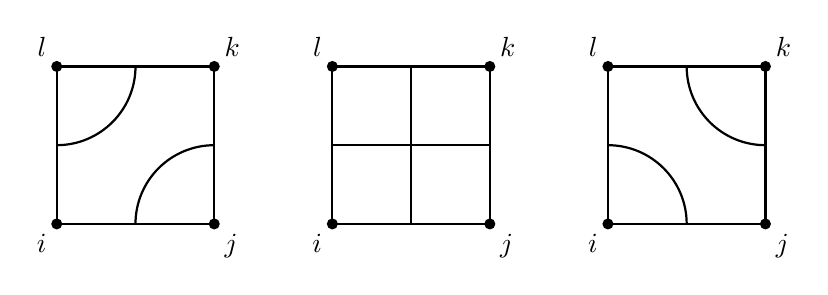
\begin{tikzpicture}[scale=1, thick]
				% ---- basic parameters ----
				\def\s{2}   % side length of one square
		\def\gap{1.5} % horizontal gap between squares

				% ===== left square =====
				\begin{scope}[shift={({-2*(\s+\gap)},0)}]
						\draw (0,0) rectangle (\s,\s);
						\fill (0,0) circle(2pt) node[below left]  {$i$};
						\fill (\s,0) circle(2pt) node[below right] {$j$};
						\fill (\s,\s) circle(2pt) node[above right] {$k$};
						\fill (0,\s) circle(2pt) node[above left]  {$l$};
						% internal quarter–circles (opposite orientation)
						\draw (0,\s/2)  arc (270:360:{\s/2});
						\draw (\s/2,0) arc (180: 90:{\s/2});
				\end{scope}


				% ===== middle square =====
				\begin{scope}[shift={({-\s-\gap},0)}]
						\draw (0,0) rectangle (\s,\s);
						\fill (0,0) circle(2pt) node[below left]  {$i$};
						\fill (\s,0) circle(2pt) node[below right] {$j$};
						\fill (\s,\s) circle(2pt) node[above right] {$k$};
						\fill (0,\s) circle(2pt) node[above left]  {$l$};
						% grid
						\draw (\s/2,0) -- (\s/2,\s);
						\draw (0,\s/2) -- (\s,\s/2);
				\end{scope}



						% ===== right square =====
				\draw (0,0) rectangle (\s,\s);
				% corner dots & labels
				\fill (0,0) circle(2pt) node[below left]  {$i$};
				\fill (\s,0) circle(2pt) node[below right] {$j$};
				\fill (\s,\s) circle(2pt) node[above right] {$k$};
				\fill (0,\s) circle(2pt) node[above left]  {$l$};
				% internal quarter–circles
				\draw (0,\s/2)  arc ( 90:  0:{\s/2});
				\draw (\s/2,\s) arc (180:270:{\s/2});
		\end{tikzpicture}
		\caption{The three ways to glue edges of a square to make an orientable surface: two spheres (left and right) and one torus (center).}
		\label{fig:square-gluings}
\end{figure}
\end{example}

The boundary of the $2n$-gon becomes a graph embedded into the
surface. It has exactly $n$ edges and one face. It may have different number
of vertices, and thus the number of vertices uniquely determines the genus of the surface:
\begin{equation*}
	V - E + F = 2 - 2g \implies g = \frac{n+1-V}{2}.
\end{equation*}
In the case of the square ($n=2$), we have $V=3$ and $g=0$ for the sphere,
and $V=1$ and $g=1$ for the torus.

\begin{figure}[htbp]
		\centering
		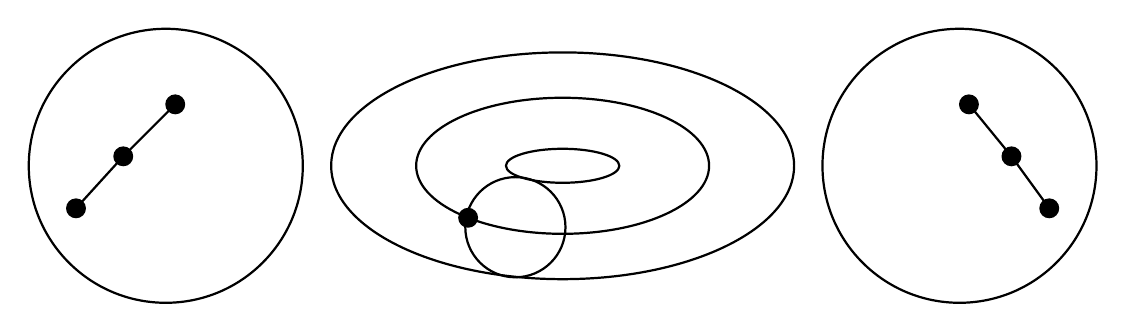
\begin{tikzpicture}[thick,scale=1.2]
				% -------------------------------------------------------------
				% handy parameters
				\def\R{1.45}   % radius of each disk
				\def\G{4.2}    % horizontal gap between the three pictures
				% -------------------------------------------------------------
				% === LEFT DISK =================================================
				\begin{scope}[shift={(-\G,0)}]
						\draw (0,0) circle (\R);
						% three collinear points and the poly‑line between them
						\coordinate (A) at (-0.95,-0.45);
						\coordinate (B) at (-0.45, 0.10);
						\coordinate (C) at ( 0.10, 0.65);
						\draw (A) -- (B) -- (C);
						\foreach \P in {A,B,C}{\fill (\P) circle(3pt);}
				\end{scope}

				% === MIDDLE TORUS (CROSS‑SECTION) =============================
				\begin{scope}
						% outer and inner “rings”
						\draw (0,0) ellipse (2.45 and 1.20);
						\draw (0,0) ellipse (1.55 and 0.72);
						% central hole (top rim)
						\draw (0,0) ellipse (0.60 and 0.18);
						% base‑point on the interior boundary
						\coordinate (P) at (-1.0,-0.55);
						\fill (P) circle(3pt);
			\draw (-.5,-.65) circle (0.53);
				\end{scope}

				% === RIGHT DISK ===============================================
				\begin{scope}[shift={(\G,0)}]
						\draw (0,0) circle (\R);
						% mirror‑image of the left‑hand poly‑line
						\coordinate (A) at ( 0.10, 0.65);
						\coordinate (B) at ( 0.55, 0.10);
						\coordinate (C) at ( 0.95,-0.45);
						\draw (A) -- (B) -- (C);
						\foreach \P in {A,B,C}{\fill (\P) circle(3pt);}
				\end{scope}
		\end{tikzpicture}
		\caption{Surfaces corresponding to gluings: left and right show three-vertex trees (disk, sphere), center shows a one-vertex, one-face case (torus).}
		\label{fig:dual-graphs-gluings}
\end{figure}

\subsection{Starting to count}

\begin{proposition}
	There is a total
	\begin{equation*}
		(2n-1)!!=(2n-1)(2n-3)\cdots 3\cdot 1
	\end{equation*}
	ways to glue the edges of a $2n$-gon into a surface.
\end{proposition}
\begin{proof}
	This is just the number of ways to pair $2n$ edges of the polygon.
\end{proof}

\begin{proposition}
	\label{prop:gluing_sphere}
	The following are equivalent:
	\begin{enumerate}
		\item The surface is a sphere;
		\item The graph on the surface is a tree;
		\item The identification of the opposite edges of the polygon is a \emph{noncrossing pairing} of the edges of the polygon.
	\end{enumerate}
\end{proposition}
\begin{proof}
	See Problem~\ref{prob:gluing_sphere}.
\end{proof}
There is $\mathrm{Cat}_n=\frac{1}{n+1}\binom{2n}{n}$ ways to get the sphere.


\subsection{Dual picture}

In the dual picture, we can consider a star with $2n$ half-edges. Then, we get a dual graph on the
same surface. This graph has $V^*=1$, $E^*=n$, but can have a variable number of faces (which corresponds to the genus):
\begin{equation*}
	F^*=n-2g+1.
\end{equation*}
When $n=2$, for the sphere, we have $F^*=3$, and for the torus, we have $F^*=1$.


\subsection{Notation}

Let us denote
\begin{align}
	\label{eq:epsg-def}
	\varepsilon_g(n)
	&\coloneqq\text{number of ways to glue the edges of a $2n$-gon into a surface of genus $g$},\\
	\label{eq:Tn-def}
	T_n(N)
	&\coloneqq
	\sum_{\text{gluings }\sigma}N^{V(\sigma)}
	=
	\sum_{g=0}^{\infty}\varepsilon_g(n)N^{n+1-2g},
\end{align}
that is, this is the generating function
of the gluings of the edges of a $2n$-gon, where
$N$ is the generating function variable.

\begin{remark}
The polynomial $T_n(N)$ has only powers of $N$ of the same parity as $n$.
\end{remark}

We have the first few polynomials
(the case $n=2$ corresponds to the square):
\begin{align*}
	T_1(N)&=N^2;\\
	T_2(N)&=2N^3+N;\\
	T_3(N)&=5N^4+10N^2;\\
	T_4(N)&=14N^5+70N^3+21N;\\
	T_5(N)&=42N^6+420N^4+483N^2.
\end{align*}

\section{Harer–Zagier formula (statement)}


Introduce the \emph{exponential generating function}
for the sequence $\{T_n(N)\}_{n\ge 0}$:
\begin{equation}\label{eq:TNs-def} % (3.1)
  \begin{split}
    T(N,s)\;=&\;1+2Ns
            +2s\sum_{n\ge 1}\frac{T_n(N)}{(2n-1)!!}\,s^{n}
        \\
       =&\;
        1+2Ns+2N^{2}s^{2}
        +\frac{2}{3}\bigl(2N^{3}+N\bigr)s^{3}
        +\frac{2}{15}\bigl(5N^{4}+10N^{2}\bigr)s^{4}
        +\dots
  \end{split}
\end{equation}

One of the goals of today's lecture is to prove the following:
\begin{theorem}
	[Harer–Zagier formula \cite{harer1986euler}]
	\label{thm:HZ-genfun}
	For every $N\in\mathbb{Z}_{>0}$ one has the closed form
\begin{equation}\label{eq:TNs-closed}
  T(N,s)\;=\;\Bigl(\frac{1+s}{1-s}\Bigr)^{N}.
\end{equation}
\end{theorem}


Let us at least
verify that
the first few Taylor coefficients of~\eqref{eq:TNs-closed}
indeed coincide with those in~\eqref{eq:TNs-def}.
Write
\begin{align*}
  \Biggl(\frac{1+s}{1-s}\Biggr)^N
  &= (1+s)^N (1-s)^{-N} \\
  &=
  \Biggl(1 + Ns + \frac{N(N-1)}{2!}s^2 + \frac{N(N-1)(N-2)}{3!}s^3 + \dots\Biggr) \\
  &\qquad\times
  \Biggl(1 + Ns + \frac{N(N+1)}{2!}s^2 + \frac{N(N+1)(N+2)}{3!}s^3 + \dots\Biggr).
\end{align*}
Multiplying the two series and collecting terms up to $s^3$, we find
\[
  1 + 2N s + 2N^2 s^2 + \frac{2}{3}(2N^3 + N) s^3 + \dots,
\]
which matches the expansion~\eqref{eq:TNs-def} exactly.




\begin{corollary}\label{cor:HZ-recurrence} % 3.1.6
For all $g\ge 0$ and $n\ge 0$, the numbers $\varepsilon_g(n)$ obey
\begin{equation}\label{eq:HZ-rec} % (3.2)
  (n+2)\,\varepsilon_g(n+1)
  \;=\;
  (4n+2)\,\varepsilon_g(n)
  \;+\;
  (4n^{3}-n)\,\varepsilon_{g-1}(n-1),
\end{equation}
with the initial condition
\[
  \varepsilon_g(0)
  \;=\;
  \begin{cases}
    1,& g=0,\\[4pt]
    0,& g\ge 1.
  \end{cases}
\]
\end{corollary}
\begin{proof}
	Follows from the identity
	\begin{equation*}
		\left( \frac{1+s}{1-s} \right)^{N}=
		(1+s)(1+s+s^2+\ldots )\left( \frac{1+s}{1-s} \right)^{N-1}.
	\end{equation*}
\end{proof}

\begin{corollary}\label{cor:epsg-explicit}
The number $\varepsilon_g(n)$ can be written as
\[
\varepsilon_g(n)\;=\;\frac{(2n)!}{(n+1)!\,(n-2g)!}\,
\bigl[s^{2g}\bigr]\!
\left(\frac{s/2}{\tanh(s/2)}\right)^{n+1},
\]
where $\bigl[s^{2g}\bigr]f(s)$ denotes the coefficient of $s^{2g}$ in the power‑series expansion of $f(s)$.
\end{corollary}



One can define another family of coefficients:
\begin{equation*}
	C_g(n)\coloneqq \frac{2^g \varepsilon_g(n)}{\mathrm{Cat}_n}.
\end{equation*}
Then, \eqref{eq:HZ-rec} can be rewritten as
\begin{equation*}
	C_g(n+1)=C_g(n)+\binom{n+1}2 C_{g-1}(n-1).
\end{equation*}
In particular, $C_g(n)$ is a positive integer, which is not straightforward from the
definition of $\varepsilon_g(n)$.


\section{Gaussian integrals and Wick formula}

\label{sec:gaussian-wick}

\subsection{The standard one–dimensional Gaussian measure}
\label{subsec:1d-gaussian}

Denote by
\[
  d\mu(x)\;=\;\frac{1}{\sqrt{2\pi}}\,
               e^{-\frac{x^{2}}{2}}\,dx,
  \qquad x\in\Bbb R,
\]
the \emph{standard centred Gaussian measure}.
We record the elementary facts that will be used repeatedly:

\begin{enumerate}[(i)]
  \item \textbf{Normalization:}
        $\displaystyle\int_{\Bbb R}d\mu(x)=1$.

  \item \textbf{Odd moments vanish:}
        $\langle x^{2n+1}\rangle=0$.

  \item \textbf{Even moments:}
        \[
          \langle x^{2n}\rangle
          \;=\;
          \frac{1}{\sqrt{2\pi}}
          \int_{-\infty}^{\infty}
            x^{2n}e^{-\frac{x^{2}}{2}}dx
          \;=\;(2n-1)!!,
          \qquad n\in\Bbb N.
        \]

  \item \textbf{Characteristic (Fourier–Laplace) transform:}
        \[
          \varphi(t)
          \;=\;
          \int_{\Bbb R}e^{itx}\,d\mu(x)
          \;=\;
          e^{-\frac{t^{2}}{2}},
          \qquad t\in\Bbb R.
        \]
\end{enumerate}
Here and below we use the convenient bracket notation
\(
  \langle f\rangle:=\int_{\Bbb R}f(x)\,d\mu(x)
\)
for expectations.



\begin{example}
\label{ex:x4}
For $k=1$ with variance~$1$ we have
\(
  \langle x^{4}\rangle
  = 3\,\langle x^{2}\rangle^{2}=3.
\)
For degree $6$ one finds
\(
  \langle x^{6}\rangle = 15.
\)
More generally,
$\langle x^{2n}\rangle=(2n-1)!!$.
This can be computed by a simple induction.
\end{example}



\subsection{Gaussian measures on \texorpdfstring{$\Bbb R^{k}$}{Rk}}
\label{subsec:multivariate-gaussian}

Fix a positive–definite symmetric matrix
$B\in\operatorname{Sym}_{k}^{+}(\Bbb R)$ and set
$C:=B^{-1}$.
The centred Gaussian measure with covariance~$C$ is
\begin{equation}
  d\mu_{B}(x)
  \;=\;
  \underbrace{\bigl[(2\pi)^{-k/2}(\det B)^{1/2}\bigr]}_{\displaystyle =:\;Z_{B}^{-1}}
  \exp\!\Bigl(-\tfrac12\langle Bx,x\rangle\Bigr)\,d^{k}x,
  \qquad x\in\Bbb R^{k}.
  \label{eq:multivariate-gaussian-density}
\end{equation}
Orthogonal diagonalisation of~$B$ shows that the normalising
prefactor indeed gives $\int_{\Bbb R^{k}}d\mu_{B}=1$.

\paragraph{Basic facts.}
\begin{align}
  \langle x_{i}\rangle &= 0,
  \quad
  1\le i\le k;
  \label{eq:mean-zero}\\
  \langle x_{i}x_{j}\rangle &= C_{ij},
  \quad
  1\le i,j\le k.
  \label{eq:covariance}
\end{align}
All higher moments are expressed in terms of the matrix~$C$
via Wick’s formula in \Cref{subsec:wick} below.

\begin{remark}
	In this lecture, we consider only \emph{centered} (mean zero) Gaussian measures.
\end{remark}

\subsection{Wick (Isserlis) formula}
\label{subsec:wick}

The essence of Wick’s formula is that \emph{every} moment of a
centred Gaussian vector is a sum over pairwise contractions governed
solely by the covariance matrix.

\begin{theorem}[Wick’s (or Isserlis’) formula]
\label{thm:wick}
Let $x=(x_{1},\dots,x_{k})$ be distributed according
to~\eqref{eq:multivariate-gaussian-density}.
For an integer $n\ge1$ and indices $i_{1},\dots,i_{2n}\in\{1,\dots,k\}$,
\begin{equation}
  \bigl\langle x_{i_{1}}\cdots x_{i_{2n}}\bigr\rangle
  \;=\;
  \sum_{p\in\operatorname{Pair}(2n)}
        \;\prod_{\{a,b\}\in p}
        C_{i_{a}i_{b}},
  \label{eq:wick}
\end{equation}
where $\operatorname{Pair}(2n)$ is the set of all
$(2n-1)!!$ perfect pairings of $\{1,\dots,2n\}$.
If the degree is \emph{odd}, then the expectation vanishes.

More generally, for any \emph{linear} functions (not necessarily distinct)
$f_1,\ldots,f_{2n}$ of the variables $x_1,\ldots,x_k$, we have
\begin{equation}
	\label{eq:f_Wick}
	\bigl\langle f_{1}\cdots f_{2n}\bigr\rangle
	=\sum
	\langle f_{p_1}f_{q_1} \rangle
	\langle f_{p_2}f_{q_2} \rangle \ldots
	\langle f_{p_n}f_{q_n} \rangle,
\end{equation}
where the sum is over all pairings of the indices $1,\ldots,2n$,
and $p_1<p_2<\ldots<p_n$ , $q_1<q_2<\ldots<q_n$ are the
indices encoding the pairing.
\end{theorem}

\begin{proof}[Sketch of proof]
	When $C=\operatorname{diag}(\sigma_{1}^{2},\dots,\sigma_{k}^{2})$,
mixed covariances vanish and Wick’s formula factorizes:
\begin{equation*}
  \bigl\langle
     x_{1}^{2n_{1}}\cdots x_{k}^{2n_{k}}
  \bigr\rangle
  \;=\;
  \prod_{i=1}^{k}
    (2n_{i}-1)!!\;\sigma_{i}^{2n_{i}},
  \qquad n_{1},\dots,n_{k}\in\Bbb N.
  \label{eq:wick-diagonal}
\end{equation*}
Indeed, pairings are allowed only between indices of the same variable,
and then the number of pairings within one variable $x_i$ is $(2n_i-1)!!$.

The general case of Wick’s formula follows from the diagonal case by
making a linear change of variables which diagonalizes the covariance matrix, and using the linearity of
\eqref{eq:f_Wick}.
\end{proof}

\begin{example}
	The one-dimensional integral
	$\langle  x^4 \rangle =\frac{1}{\sqrt{2\pi}} \int_{-\infty}^{\infty} x^4 e^{-\frac{x^2}{2}} dx$ can be computed using Wick’s formula:
	\begin{equation*}
		\langle f_1f_2f_3f_4 \rangle =
		\langle f_1f_2 \rangle \langle f_3f_4 \rangle + \langle f_1f_3 \rangle \langle f_2f_4 \rangle + \langle f_1f_4 \rangle \langle f_2f_3 \rangle,
	\end{equation*}
	where $f_i(x)=x$ for $i=1,2,3,4$.
	We know this integral is equal to $3$.
\end{example}

\begin{remark}
	\label{rem:wick-linear}
	Note that in the second part of \Cref{thm:wick},
	the linear functions $f_j$ must be not \emph{affine}, but truly \emph{linear},
	that is, $f_j(0,\ldots,0)=0$. See Problem~\ref{prob:wick-linear}.
\end{remark}


\section{GUE integrals and gluing polygons}

We will now apply Wick’s formula to compute the moments of traces of
GUE matrices. Recall that in
\href{https://lpetrov.cc/rmt25/rmt25-notes/rmt2025-l01.pdf}{Lecture 1}
and
\href{https://lpetrov.cc/rmt25/rmt25-notes/rmt2025-l02.pdf}{Lecture 2} we
worked with general Wigner matrices (real symmetric or Hermitian),
and now we will deal with the special case of
GUE, Gaussian Hermitian matrices.
Here, the Gaussian distribution will allow us to
connect the moments of traces of GUE matrices to the topology of surfaces.

\subsection{Traces of powers, again}
\label{subsec:traces-powers}


Let $\mathcal{H}_N$ be the space of $N\times N$ Hermitian matrices,
and $\mu$ on $\mathcal{H}_N$ be the GUE measure, with complex variances $1$
for the diagonal and off-diagonal entries.
Let us begin by an example with $n=2$.

Consider the integral
\[
  \int_{\mathcal{H}_N}\!\operatorname{tr}(H^4)\,d\mu(H).
\]
Here the integrand is a sum of monomials,
\[
  \operatorname{tr}(H^4)
  \;=\;
  \sum_{i,j,k,l=1}^N
    h_{ij}\,h_{jk}\,h_{kl}\,h_{li}.
\]
Since each entry $h_{pq}$ is a linear function of the real and imaginary parts
of $H$, we may apply Wick’s formula:
\begin{equation}\label{eq:wick-square}
  \bigl\langle h_{ij}h_{jk}h_{kl}h_{li}\bigr\rangle
  =
  \langle h_{ij}h_{jk}\rangle\,\langle h_{kl}h_{li}\rangle
  +
  \langle h_{ij}h_{kl}\rangle\,\langle h_{jk}h_{li}\rangle
  +
  \langle h_{ij}h_{li}\rangle\,\langle h_{jk}h_{kl}\rangle.
\end{equation}
\begin{lemma}
	We have $\langle h_{ij}h_{ji} \rangle =1$, and all other
	second moments are zero.
\end{lemma}
\begin{proof}
	This is straightforward from the independence of real and imaginary parts of the entries of $H$.
\end{proof}

Let us inspect each term in \eqref{eq:wick-square} separately:
\begin{itemize}
  \item In the first product
        $\langle h_{ij}h_{jk}\rangle$ is nonzero only when $i=k$, and then equals $1$.
        Likewise $\langle h_{kl}h_{li}\rangle=1$ only when $k=i$.  Summing over all $i,j,k,l$
        with $i=k$ gives $N^3$.

  \item In the second product
        $\langle h_{ij}h_{kl}\rangle\,\langle h_{jk}h_{li}\rangle$ is nonzero
        only if $i=j=k=l$, and then each factor equals $1$.  Hence this term contributes $N$.

  \item The third product is identical in structure to the first and therefore contributes another $N^3$.
\end{itemize}
There is a one‐to‐one correspondence between these three terms in \eqref{eq:wick-square}
and the three pairings of the edges of a square (see \Cref{fig:square-gluings}).  Each pairing contributes
$N^{V(\sigma)}$, where $V(\sigma)$ is the number of vertices in the glued graph.

Putting everything together, we get
\[
  \int_{\mathcal{H}_N}\!\operatorname{tr}(H^4)\,d\mu(H)
  \;=\;
  2\,N^3 + N
  \;=\;
	T_2(N),
\]
where $T_2(N)$ is defined by \eqref{eq:Tn-def}.

In a similar manner, we obtain the following:
\begin{proposition}
	\label{prop:traces-moments}
	For any $n\ge 1$, we have
	\[
		\int_{\mathcal{H}_N}\!\operatorname{tr}(H^{2n})\,d\mu(H)
		\;=\;
		T_n(N).
	\]
	Odd moments (expectations of $\operatorname{tr}(H^{2n+1})$) vanish.
\end{proposition}
\begin{proof}[Proof sketch]
	The idea why we get the genus will be evident from a larger example.
	Let $n=4$, so we are dealing with a sum of $N^{8}$ monomials of the form
\[
  h_{i_{1}i_{2}}
  h_{i_{2}i_{3}}
  h_{i_{3}i_{4}}
  h_{i_{4}i_{5}}
  h_{i_{5}i_{6}}
  h_{i_{6}i_{7}}
  h_{i_{7}i_{8}}
  h_{i_{8}i_{1}}.
\]
Choose an arbitrary Wick pairing (there are $7!!=105$ of them).
For instance, pair
\[
  h_{i_{1}i_{2}}\;\text{with}\;h_{i_{4}i_{5}},\quad
  h_{i_{2}i_{3}}\;\text{with}\;h_{i_{5}i_{6}},\quad
  h_{i_{3}i_{4}}\;\text{with}\;h_{i_{8}i_{1}},\quad
  h_{i_{6}i_{7}}\;\text{with}\;h_{i_{7}i_{8}}.
\]
In other words, consider the product
\begin{equation}
  \bigl\langle h_{i_{1}i_{2}}h_{i_{4}i_{5}}\bigr\rangle
  \bigl\langle h_{i_{2}i_{3}}h_{i_{5}i_{6}}\bigr\rangle
  \bigl\langle h_{i_{3}i_{4}}h_{i_{8}i_{1}}\bigr\rangle
  \bigl\langle h_{i_{6}i_{7}}h_{i_{7}i_{8}}\bigr\rangle.
  \label{eq:example-3.10}
\end{equation}
Each factor in
\eqref{eq:example-3.10} is usually~$0$; if any of them vanishes, so does
the whole product.  For the product to be non–zero, \emph{every} factor
must equal~$1$, which imposes the constraints
\[
  \langle h_{i_{1}i_{2}}h_{i_{4}i_{5}}\rangle = 1
  \iff
  i_{1}=i_{5},\; i_{2}=i_{4};
\qquad
  \langle h_{i_{2}i_{3}}h_{i_{5}i_{6}}\rangle = 1
  \iff
  i_{2}=i_{6},\; i_{3}=i_{5};
\]
\[
  \langle h_{i_{3}i_{4}}h_{i_{8}i_{1}}\rangle = 1
  \iff
  i_{3}=i_{1},\; i_{4}=i_{8};
\qquad
  \langle h_{i_{6}i_{7}}h_{i_{7}i_{8}}\rangle = 1
  \iff
  i_{6}=i_{8},\; i_{7}=i_{7}.
\]
Altogether we obtain the \emph{chain of equalities}
\[
  i_{1}=i_{5}=i_{3}=i_{1},\qquad
  i_{2}=i_{4}=i_{8}=i_{6}=i_{2},\qquad
  i_{7}=i_{7},
\]
which leaves $i_{1},i_{2},i_{7}$ free and therefore yields $N^{3}$
admissible index choices.  So, the contribution of the pairing
\eqref{eq:example-3.10} equals $N^{3}$.

\medskip
Now, 
consider an octagon ($2n=8$), and glue its sides in pairs as illustrated in
Figure~\ref{fig:octagon-gluing}.  Writing, for example,
\[
  i_{1}=i_{5},\; i_{2}=i_{4},\qquad
  i_{2}=i_{6},\; i_{3}=i_{5},\qquad
  i_{3}=i_{1},\; i_{4}=i_{8},\qquad
  i_{6}=i_{8},
\]
we see that the eight initial vertices collapse into
\[
  i_{1}=i_{5}=i_{3},\quad
  i_{2}=i_{4}=i_{6}=i_{8},\quad
  i_{7}=i_{7},
\]
producing $V(\sigma)=3$ vertices in the resulting map; hence the gluing
$\sigma$ shown in Figure~\ref{fig:octagon-gluing} contributes
$N^{V(\sigma)} = N^{3}$.


\begin{figure}[htbp]
  \centering


  \caption{An $8$–gon with pairwise–identified sides corresponding to the
           Wick pairing.}
  \label{fig:octagon-gluing}
\end{figure}
\end{proof}








\section{Multi-matrix models}



\section{Two-matrix models and the Ising model}




























\appendix
\setcounter{section}{14}

\section{Problems (due 2025-04-29)}

\subsection{Gluing a Sphere}
\label{prob:gluing_sphere}
Show that for a connected, orientable surface formed by gluing the edges of a $2n$-gon in pairs, the following are equivalent:
\begin{enumerate}
	\item The resulting surface is a sphere.
	\item The embedded graph formed by the identification is a tree.
	\item The pairing of edges corresponds to a \emph{noncrossing pairing} (i.e., when the edges are arranged around the polygon in order, the identifications can be drawn inside the disk without crossings).
\end{enumerate}
(This is the proof of \Cref{prop:gluing_sphere}.)

\subsection{Wick's formula for affine functions}
\label{prob:wick-linear}
Consider the integrals of the form
\[
	I(a_1, \ldots, a_k) := \int_{-\infty}^\infty \prod_{i=1}^k (x - a_i)\; \frac{1}{\sqrt{2\pi}} e^{-x^2/2}\, dx,
\]
where $a_1, \ldots, a_k \in \mathbb{R}$ are fixed parameters.

Compute $I(a_1, a_2)$ and $I(a_1, a_2, a_3, a_4)$ explicitly as polynomials in $a_1,\ldots, a_4$,
and compare $I(a_1, a_2, a_3, a_4)$ with the Wick-like expansion.




\bibliographystyle{alpha}
\bibliography{bib}


\medskip

\textsc{L. Petrov, University of Virginia, Department of Mathematics, 141 Cabell Drive, Kerchof Hall, P.O. Box 400137, Charlottesville, VA 22904, USA}

E-mail: \texttt{lenia.petrov@gmail.com}


\end{document}
